% =====================================================================
% AI Academy -- National AI Center
% Software Engineering Final Project -- Team Presentation Deck
% Topic 4: Async Research Assistant
% Compile with pdfLaTeX (Overleaf works out of the box).
% =====================================================================

\PassOptionsToPackage{dvipsnames}{xcolor}
\documentclass[aspectratio=169,11pt]{beamer}

% ===== CONFIGURATION =================================================
\newcommand{\teamname}{Topic Four}
\newcommand{\topicchoice}{Topic 4 -- Async Research Assistant}
\newcommand{\memberone}{Nural Shukurlu}
\newcommand{\membertwo}{Emil Mammadov}
\newcommand{\memberthree}{Mahammadali Babayev}
\newcommand{\memberfour}{Bailar Bayramov}
\newcommand{\repolink}{github.com/nuralnetworks/async-research-assistant}

\newcommand{\coursecode}{AI-ENG-110}
\newcommand{\coursename}{Software Engineering}
\newcommand{\institution}{AI Academy, National AI Center}
\newcommand{\semester}{Spring 2026}

% ===== PACKAGES ======================================================
\usepackage[T1]{fontenc}
\usepackage[utf8]{inputenc}
\usepackage{xcolor}
\usepackage{tabularx}
\usepackage{booktabs}
\usepackage{listings}
\usepackage{tikz}
\usetikzlibrary{shapes.geometric,arrows.meta,positioning,fit,backgrounds}

% ===== BEAMER THEME ==================================================
\usetheme{default}
\usefonttheme{professionalfonts}
\setbeamertemplate{navigation symbols}{}

\definecolor{accent}{HTML}{0B3D91}
\definecolor{soft}{HTML}{F2F4F8}
\definecolor{ok}{HTML}{166534}

\setbeamercolor{title}{fg=accent}
\setbeamercolor{frametitle}{fg=accent}
\setbeamercolor{section in head/foot}{bg=accent,fg=white}
\setbeamercolor{itemize item}{fg=accent}
\setbeamercolor{itemize subitem}{fg=accent}
\setbeamercolor{enumerate item}{fg=accent}
\setbeamercolor{block title}{bg=accent,fg=white}
\setbeamercolor{block body}{bg=soft,fg=black}

\setbeamerfont{title}{size=\Large,series=\bfseries}
\setbeamerfont{frametitle}{size=\large,series=\bfseries}
\setbeamerfont{footline}{size=\tiny}

\setbeamertemplate{footline}{%
  \leavevmode%
  \hbox{\hspace*{2ex}\tiny\textit{\teamname{} -- \topicchoice}\hfill%
  \tiny\textit{\coursecode{} -- \semester{}}\hfill%
  \tiny\insertframenumber/\inserttotalframenumber\hspace*{2ex}}%
  \vskip1pt%
}

% ===== CODE LISTINGS =================================================
\definecolor{codegreen}{rgb}{0,0.55,0}
\definecolor{codepurple}{rgb}{0.55,0,0.78}
\lstdefinestyle{python}{
  language=Python,
  backgroundcolor=\color{soft},
  commentstyle=\color{codegreen},
  keywordstyle=\color{accent},
  stringstyle=\color{codepurple},
  basicstyle=\ttfamily\scriptsize,
  breaklines=true,
  frame=single,
  framerule=0.4pt,
  rulecolor=\color{black!30},
}

% =====================================================================
\begin{document}

% ========== SLIDE 1: TITLE ===========================================
{%
\setbeamertemplate{footline}{}
\begin{frame}[plain]
  \begin{center}
    \vspace{0.6cm}
    {\small \textsc{\institution}}\\[0.2em]
    {\small \textsc{\coursecode{} -- \coursename{} -- \semester{}}}\\[1.2em]
    \rule{0.7\textwidth}{0.6pt}\\[0.4em]
    {\Huge\bfseries\color{accent} \topicchoice}\\[0.4em]
    \rule{0.7\textwidth}{0.6pt}\\[1.2em]
    {\large \teamname}\\[0.6em]
    {\normalsize \memberone\quad\textbullet\quad\membertwo\quad\textbullet\quad\memberthree\quad\textbullet\quad\memberfour}\\[1cm]
    {\footnotesize\itshape Final Project Defense -- September 2026}\\[0.4em]
    {\footnotesize\texttt{\repolink}}
  \end{center}
\end{frame}
}

% ========== SLIDE 2: PROBLEM =========================================
\begin{frame}{The problem in one sentence}
  \begin{block}{What the system does}
    You ask a research question in plain language; we query Wikipedia, arXiv, and web search at the same time and return one short answer with numbered citations.
  \end{block}

  \vspace{0.3em}
  \begin{columns}[T,onlytextwidth]
  \column{0.48\textwidth}
  \textbf{Inputs}
  \begin{itemize}
    \item One question string (3--2000 chars)
    \item Optional source subset, cache flag
  \end{itemize}

  \column{0.48\textwidth}
  \textbf{Outputs}
  \begin{itemize}
    \item Answer text with [N] citations
    \item Reference list: title + URL + origin
  \end{itemize}
  \end{columns}

  \vspace{0.4em}
  \textbf{Entry points:} \texttt{ask}, \texttt{demo}, \texttt{bench} under \texttt{python -m researcher} (plus \texttt{--offline} for keyless runs)
\end{frame}

% ========== SLIDE 3: ARCHITECTURE ====================================
\begin{frame}{Architecture}
  \textbf{Module map.} Only the service layer touches the \emph{provided} \texttt{ai/} package.

  \vspace{0.3em}
  \begin{center}
  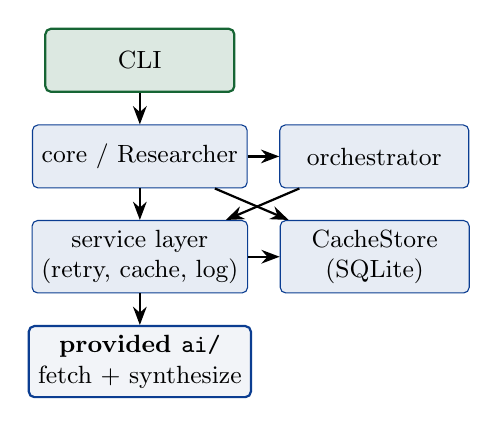
\begin{tikzpicture}[
    node distance=4mm,
    box/.style={draw,rounded corners=2pt,minimum width=2.4cm,minimum height=0.8cm,align=center,font=\small},
    aibox/.style={box,fill=soft,draw=accent,thick},
    sebox/.style={box,fill=accent!10,draw=accent},
    entry/.style={box,fill=ok!15,draw=ok,thick},
    arrow/.style={-Stealth,thick}
  ]
    \node[entry] (cli) {CLI};
    \node[sebox,below=of cli] (core) {core / Researcher};
    \node[sebox,right=of core] (conc) {orchestrator};
    \node[sebox,below=of core] (svc)  {service layer\\(retry, cache, log)};
    \node[sebox,right=of svc] (store) {CacheStore\\(SQLite)};
    \node[aibox,below=of svc] (ai) {\textbf{provided \texttt{ai/}}\\fetch + synthesize};
    \draw[arrow] (cli) -- (core);
    \draw[arrow] (core) -- (conc);
    \draw[arrow] (core) -- (svc);
    \draw[arrow] (conc) -- (svc);
    \draw[arrow] (svc) -- (ai);
    \draw[arrow] (svc) -- (store);
    \draw[arrow] (core) -- (store);
  \end{tikzpicture}
  \end{center}

  \vspace{0.3em}
  {\footnotesize\textit{Swapping Gemini for OpenAI touches one file plus \texttt{.env}. Pydantic models everywhere; no plain dicts cross modules.}}
\end{frame}

% ========== SLIDE 4: KEY DESIGN DECISIONS ============================
\begin{frame}{Three design decisions we can defend}
  \begin{enumerate}\setlength\itemsep{0.6em}
    \item \textbf{\texttt{asyncio} over threads}\\
      Three independent network waits; threads add risk for no gain, processes would be absurd for HTTP.
    \item \textbf{Cache behind an ABC, service built by composition}\\
      SQLite swaps for files without touching callers; the service \emph{uses} a store instead of inheriting one.
    \item \textbf{SQLite file over a database server}\\
      Zero infrastructure, reproducible grading, honest trade: single-writer only.
  \end{enumerate}
\end{frame}

% ========== SLIDE 5: CONCURRENCY (THE BENCHMARK) =====================
\begin{frame}{Concurrency: the benchmark}
  \textbf{Workload:} 5 questions $\times$ 3 sources (15 fetches, 300\,ms simulated each), cleared cache, \texttt{scripts/bench.py --offline}

  \vspace{0.4em}
  \begin{center}\small
  \begin{tabular}{lcc}
    \toprule
    & \textbf{Sequential} & \textbf{Concurrent (sem=3)} \\
    \midrule
    Wall-clock (s) & 4.52 & 2.73 \\
    Speedup        & 1.0$\times$ & 1.66$\times$ \\
    Provider 429s  & 0  & 0 \\
    \bottomrule
  \end{tabular}
  \end{center}

  \vspace{0.4em}
  \textbf{Bottleneck named:} our own token bucket plus the single serial synthesis call\\
  \textbf{What didn't reach $N\times$:} Sleeps dominate equally in both modes; the bucket caps bursts by design
\end{frame}

% ========== SLIDE 6: ROBUSTNESS STORY ================================
\begin{frame}{Robustness: the stale-cache incident}
  \textbf{Scenario:} a demo answered ``photosynthesis'' with physics papers and zero Wikipedia hits

  \vspace{0.3em}
  \textbf{How we surfaced it:} cache-hit logs showing zero items; empty hits cached with a 24h TTL kept re-serving

  \vspace{0.3em}
  \textbf{What the system does now:}
  \begin{itemize}\setlength\itemsep{0.3em}
    \item Retry: 3 attempts, exponential backoff 1--8\,s plus jitter (transient errors only)
    \item Shape: keywords for Wikipedia/arXiv, full sentences for web search
    \item Cache: never store empties; versioned keys orphan old logic
    \item Degrade: one dead source becomes a warning, never a crash
  \end{itemize}
\end{frame}

% ========== SLIDE 7: DEMO ============================================
\begin{frame}[fragile]{Live demo (or scripted demo)}
  \begin{block}{What we will run}
    One unseen question across all three live sources, then the scripted five-question digest.
  \end{block}

  \vspace{0.4em}
  \textbf{Demo command (works inside Docker):}
  \begin{lstlisting}[style=python,language=bash,numbers=none]
$ docker run --env-file .env finalproj \
    python -m researcher ask "Who was Marie Curie?"
  \end{lstlisting}

  \vspace{0.4em}
  \begin{itemize}
    \item Watch the [N] citations resolve to titles and URLs on screen.
    \item \texttt{demo --limit 5} writes \texttt{artefacts/answers.json} plus a dated digest.
  \end{itemize}

  \vspace{0.3em}
  {\footnotesize\textit{Fresh artefacts from a 5/5 live run ship in the repo. Offline mode needs no keys at all.}}
\end{frame}

% ========== SLIDE 8: TESTING =========================================
\begin{frame}{Testing}
  \begin{columns}[T,onlytextwidth]
  \column{0.55\textwidth}
  \textbf{Coverage \& shape}
  \begin{itemize}\setlength\itemsep{0.3em}
    \item Total coverage: 86\,\%
    \item Provided \texttt{ai/} smoke tests: \textcolor{ok}{\textbf{passing}} (16/16)
    \item Test count: 57 own + 16 smoke
    \item All tests offline; AI module fully mocked
  \end{itemize}

  \column{0.42\textwidth}
  \textbf{Three tests worth calling out}
  \begin{itemize}\setlength\itemsep{0.3em}
    \item Happy-path end-to-end \texttt{ask}
    \item Concurrency: one source fails, answer still lands
    \item Error path: empty hits are never cached
  \end{itemize}
  \end{columns}

  \vspace{0.6em}
  \begin{block}{Tooling}
    \texttt{pytest} + \texttt{pytest-asyncio} + \texttt{pytest-cov} + \texttt{respx} / \texttt{unittest.mock}. \texttt{mypy} clean on 15 files, \texttt{ruff} clean.
  \end{block}
\end{frame}

% ========== SLIDE 9: LIMITATIONS + FUTURE ============================
\begin{frame}{Limitations \& what we'd do next}
  \textbf{Where the system is brittle today}
  \begin{itemize}\setlength\itemsep{0.3em}
    \item No provider failover; if Gemini is down, synthesis stops with a clean error.
    \item Single-process SQLite and rate limiter; scale needs Postgres plus a shared budget.
    \item Web search is the fragile leg; DuckDuckGo throttles some networks, Tavily is the paid escape.
  \end{itemize}

  \vspace{0.4em}
  \textbf{Given another week we would}
  \begin{enumerate}\setlength\itemsep{0.3em}
    \item Add LLM failover with a chaos test killing the primary.
    \item Load-test past the benchmark harness to measure the real ceiling.
    \item Rank sources by quality so weak hits never get cited.
  \end{enumerate}
\end{frame}

% ========== SLIDE 10: TEAM CONTRIBUTIONS =============================
\begin{frame}{Team contributions}
  \begin{center}\footnotesize
  \begin{tabularx}{\linewidth}{lXl}
    \toprule
    \textbf{Member} & \textbf{Primary ownership} \\
    \midrule
    Nural Shukurlu   & models, resilient service, rate limiter, config, touch-ups   \\
    Emil Mammadov    & cache store (SQLite), parallel orchestrator                  \\
    Mahammadali Babayev & core pipeline, demo/bench scripts, artefacts           \\
    Bailar Bayramov  & CLI, Dockerfile, CI, README, report/slides assembly          \\
    \bottomrule
  \end{tabularx}
  \end{center}

  \vspace{0.4em}
  \textbf{AI tool use:} coding assistance for routine work; the team reviewed, tested, and owns everything.
\end{frame}

% ========== SLIDE 11: THANK YOU / Q&A ================================
{%
\setbeamertemplate{footline}{}
\begin{frame}[plain]
  \begin{center}
    \vspace{1cm}
    {\Huge\bfseries\color{accent} Questions?}\\[1.2em]
    \rule{0.5\textwidth}{0.6pt}\\[1.2em]
    {\large \teamname}\\[0.6em]
    {\normalsize \texttt{\repolink}}
  \end{center}
\end{frame}
}

\end{document}
